\documentclass[aspectratio=169]{beamer}
% Themes ---------------------------------------------------------------------
\usetheme{default}
\usefonttheme{professionalfonts}
% Packages -------------------------------------------------------------------
\usepackage{graphicx}
\usepackage{enumitem}
\usepackage{stmaryrd}
\usepackage[most]{tcolorbox}
\usepackage{booktabs}
\usepackage{import}
\usepackage{adjustbox}
\usepackage{MnSymbol}
\usepackage{fancyvrb}
% Tables ---------------------------------------------------------------------
\renewcommand{\arraystretch}{1.3}
% enumitem -------------------------------------------------------------------
\setlist{itemsep=10pt}
% beamer ---------------------------------------------------------------------
\setbeamerfont{caption}{size=\small}
% Title & author -------------------------------------------------------------
\title{1.1 Why Python?}
\subtitle{Getting Started}
\author{Jakob Wells}

\begin{document}
\date{\today}


\begin{frame}
    \titlepage{}
\end{frame}

\begin{frame}{Instructor details}
    \begin{table}
    \centering
        \begin{tabular}{ll}
            Instructor & Jakob Wells                      \\
            Office     & 1008                             \\
            Email      & jakob.wells@lwshanghai.org       \\
            Website    & https://gitlab.com/jakobwells/cs \\
        \end{tabular}
    \end{table}
\end{frame}


\begin{frame}{In an email:}{Classwork 01}
    \textbf{To:} \texttt{jakob.wells@lwshanghai.org} \\
    \vspace{5pt}
    \textbf{Subject:} \texttt{[CS] Classwork 01} \\
    \vspace{10pt}
    \begin{enumerate}[label={\arabic*.}]
        \item What is your Chinese name? (given name, then family name)
        \item What is your English name?
        \item What is your GitLab username?
        \item What is your homeroom?
        \item Why are you taking this class?
        \item I learn best in classes where the teacher\ldots
    \end{enumerate}
\end{frame}


\begin{frame}[fragile]{Classwork 01}{Due on 2022/09/05}
    \begin{Verbatim}[fontsize=\tiny]
To: jakob.wells@lwshanghai.org
Subject: [CS] Classwork 01
Body:
Hi Mr. Jakob,

Below are my responses for the first assignment.

1. What is your Chinese name?
Chen Li

2. What is your English name?
James

3. What is your GitLab username?
jamesli42

4. What is your homeroom?
9A

5. Why are you taking this class?
I took computer science last year and thought it was really interesting.

6. I learn best in classes where the teacher asks me questions.

Cheers,
James Li
    \end{Verbatim}
\end{frame}


\begin{frame}{Semester 1}
    \begin{table}
    \centering
        \begin{tabular}{ccl}
            \toprule
            \textbf{Approx. Dates} & \textbf{Unit} & \textbf{Topic}                  \\
            \midrule
            09.05-09.09            & 1             & Getting Started                 \\
            09.12-09.30            & 2             & Variables and Simple Data Types \\
            10.03-10.21            & 3             & Introducing Lists               \\
            10.24-11.18            & 4             & Working With Lists              \\
            11.09-11.10            & -             & Midterm Evaluation              \\
            11.21-12.16            & 5             & \texttt{if} Statements          \\
            12.19-01.13            & 6             & Dictionaries                    \\
            01.16-01.17            & -             & Final Evaluation                \\
            \bottomrule
        \end{tabular}
    \end{table}   
\end{frame}


\begin{frame}{Semester 2}
    \begin{table}
    \centering
        \begin{tabular}{ccl}
            \toprule
            \textbf{Approx. Dates} & \textbf{Unit} & \textbf{Topic}                                 \\
            \midrule
            12.12-12.23            & 7             & User Input and \texttt{while} Loops \\
            09.02-09.16            & 8             & Function \\
            09.19-10.07            & 9             & Classes \\
            10.10-10.28            & 10            & Files and Exceptions \\
            10.31-11.08            & 11            & Testing Your Code \\
            04.19-04.21            & -             & Midterm Evaluation                             \\
            11.09-11.10            & A             & Using Git for Version Control \\
            11.09-11.10            & -             & Projects \\
            06.26-06.28            & -             & Final Evaluation \\
            \bottomrule
        \end{tabular}
    \end{table}   
\end{frame}


\begin{frame}{Grade breakdown}
    \begin{table}
    \centering
        \begin{tabular}{lc}
            \toprule
            \textbf{Activity}  & \textbf{\% of grade} \\
            \midrule
            Participation      & 15\% \\
            Classwork          & 15\% \\
            Unit Evaluation    & 20\% \\
            Midterm Evaluation & 20\% \\
            Final Evaluation   & 30\% \\
            Extra Credit       & \(\leq\)5\% \\
            \bottomrule
                               & 105\% \\
        \end{tabular}
    \end{table}   
\end{frame}


\begin{frame}{Materials}
    \textbf{Required}
    \begin{itemize}[label=--]
        \item laptop (macOS or Windows)
        \item notebook (B5 or larger)
        \item pencil or blue/black pen
    \end{itemize}
    \vspace{15pt}
    \textbf{Optional}
    \begin{itemize}[label=--]
        \item mouse
        \item portable \(\geq 512\) GB SSD/HDD for automated backups
            \begin{itemize}[label=\(\blacktriangleright\),itemsep=5pt]
                \item data loss will not be a reason for a late assignment
            \end{itemize}
    \end{itemize}
\end{frame}


\begin{frame}{Class expectations (I)}
    \begin{itemize}[label=--]
        \item Minimize distractions to yourself and others
            \begin{itemize}[label=\(\blacktriangleright\),itemsep=5pt]
                \item Arrive on time
                \item Put away mobile phones and tablets
                \item Never pack up before it's time to leave
                \item Use technology for learning
            \end{itemize}
        \item Respect the learning environment
            \begin{itemize}[label=\(\blacktriangleright\),itemsep=5pt]
                \item No food or drinks (except water)
                \item Use polite speech and body language
                \item Speak when permitted
                \item No cheating
            \end{itemize}
    \end{itemize}
\end{frame}


\begin{frame}{Class expectations (II)}
    \begin{itemize}[label=--]
        \item Be prepared to learn
            \begin{itemize}[label=\(\blacktriangleright\),itemsep=5pt]
                \item Bring required materials every day
                \item Start your assignment when the bell rings
                \item Listen and follow directions
                \item Turn in work on time
                \item Make up missed work
            \end{itemize}
    \end{itemize}
\end{frame}


\begin{frame}{Class consequences}
    \begin{enumerate}[label={\arabic*.}]
        \item Verbal warning
        \item Taking away device (if applicable)
        \item Notify homeroom teacher
        \item Detention
        \item Referral to assistant principal
    \end{enumerate}
    \vspace{15pt}
    Serious or repeated offenses can, at the teacher's discretion, result in more severe consequences regardless of previous steps taken.
    Any infraction of the rules may affect your participation grade.
    It can also be cause for further action at the teacher's discretion.
\end{frame}




\begin{frame}{Who is this class for?}
    \begin{itemize}[label=--]
        \item Students who have never programmed in Python or have never programmed at all
        \item  In the Python portion, you will:
            \begin{itemize}[label=\(\blacktriangleright\),itemsep=5pt]
                \item Learn the basics of programming quickly so you can focus on interesting projects
                \item Test your understanding of new concepts by solving meaningful problems
            \end{itemize}
        \item In the robotics portion, you will:
            \begin{itemize}[label=\(\blacktriangleright\),itemsep=5pt]
                \item Design and build real robots
                \item Create autonomous robots through programming algorithms and routines
            \end{itemize}
        \item If that sounds interesting to you, you are in the right course.
    \end{itemize}
\end{frame}


\begin{frame}{So why computer science?}
    \begin{columns}
        \begin{column}{0.5\textwidth}
            \begin{itemize}[label=--]
                \item CS isn't just for programmers
                \item CS is fun
                \item There are jobs available in CS
                \item CS pays well
            \end{itemize}
        \end{column}
        \begin{column}{0.5\textwidth}
            \centering
            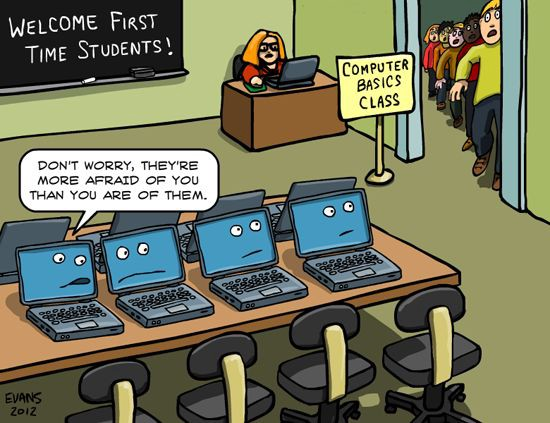
\includegraphics[width=\linewidth]{more_afraid_comic.jpg}
        \end{column}
    \end{columns}
\end{frame}


\begin{frame}{Are there jobs available?}
    \begin{itemize}[label=--]
        \item YES!
        \item \href{https://www.bls.gov/ooh/computer-and-information-technology/home.htm}{U.S. Bureau of Labor Statistics Occupational Outlook Handbook} 2020-2030
            \begin{itemize}[label=\(\blacktriangleright\)]
                \item Computer and Information Technology Occupations
                \begin{itemize}[label=--,itemsep=5pt]
                    \item projected 13\% growth
                    \item projected 667,600 new jobs
                \end{itemize}
            \end{itemize}
        \item \href{https://money.usnews.com/careers/best-jobs/rankings/the-100-best-jobs}{U.S. News 100 Best Jobs}
            \begin{itemize}[label=\(\blacktriangleright\),itemsep=5pt]
                \item \#1 - Information Security Analyst
                \item \#5 - Software Developer
                \item \#6 - Data Scientist
            \end{itemize}
    \end{itemize}
\end{frame}


\begin{frame}{Does it pay well?}
    \begin{table}
    \centering
        \begin{tabular}{lc}
            \toprule
            \textbf{Career}    & \textbf{Avg. Salary} \\
            \midrule
            National Average   & \$68,000             \\
            \midrule
            Software Engineer  & \$89,000             \\
            Data Scientist     & \$98,000             \\
            \bottomrule
        \end{tabular}
    \end{table}   
\end{frame}


\begin{frame}{How many computers do you interact with in a day?}
    \uncover<2->{\begin{itemize}[label=--]
        \item phone/tablet/laptop
        \item e-reader
        \item smart watch
        \item gaming console
        \item car
        \item cash register
        \item smart TV
    \end{itemize}}
\end{frame}


\begin{frame}{Warm-up exercise}
    \begin{itemize}[label=--]
        \item As a class, create a list of:
            \begin{itemize}[label=--,itemsep=5pt]
                \item Things that are ``computers''
                \item Tasks that can be accomplished by a computer
            \end{itemize}
        \item Come to the front of the class and add a \textit{new} entry to each list (include your name)
    \end{itemize}
    \begin{table}
    \centering
        \begin{tabular}{ll}
            \toprule
            \textbf{Things that are ``computers''} & \textbf{Tasks accomplished by a computer} \\
            \midrule
            - Smartphones (Mr. Wells)              & - Filing taxes (Mr. Wells)                           \\
            - \ldots                               & - \ldots                                             \\
        \end{tabular}
    \end{table}   
\end{frame}


\begin{frame}{What is a computer?}
    \begin{itemize}[label=--]
        \item A machine that manipulates data and executes lists of instructions known as programs.
            \begin{itemize}[label=\(\blacktriangleright\),itemsep=5pt]
                \item The same computer can perform many different tasks (depending on what program is running)
                \item A computer can be built that is capable or running programs that don't even exist yet
            \end{itemize}
        \item Made of hardware and software
            \begin{itemize}[label=\(\blacktriangleright\),itemsep=5pt]
                \item Hardware: physical components (e.g. CPU, memory, storage)
                \item Software: collection of programs (e.g. Windows, Microsoft Office, bilibili)
            \end{itemize}
        \item A \textbf{program} is a list of instructions to be carried out by a computer.
    \end{itemize}
\end{frame}


\begin{frame}{What is Computer Science?}
    \begin{itemize}[label=--]
        \item Not programming
        \item We'll study programming because it is a good way of explaining the approach that Computer Scientists take to solve problems
    \end{itemize}
\end{frame}


\begin{frame}{Programming}
    \begin{itemize}[label=--]
        \item Computer programs are also stored as 1s and 0s
            \begin{itemize}[label=\(\blacktriangleright\),itemsep=5pt]
                \item This is called \textbf{machine language}
            \end{itemize}
        \item We don't write program in 1s and 0s! (Anymore.)
            \begin{itemize}[label=\(\blacktriangleright\),itemsep=5pt]
                \item We have some mechanisms to simplify this
                \item We write text in programming languages (e.g. C++, Java, Python)
                \item A special program called a compiler turns this text into machine language
            \end{itemize}
        \item A \textbf{compiler} is a program that translates a program written in one language into an equivalent program in another language.
    \end{itemize}
\end{frame}


\begin{frame}{Creating an algorithm}
    \begin{itemize}[label=--]
        \item Think of an everyday task (e.g. baking a cake) and write an algorithm for it
        \item Does your algorithm use any \textit{loops} or \textit{conditionals}?
        \item Share your algorithm with a classmate.
            \begin{itemize}[label=\(\blacktriangleright\),itemsep=5pt]
                \item Is it sufficient for them to perform the task?
                \item Can they identify any \textit{bugs} in your algorithm?
                \item How did you debug your algorithm?
            \end{itemize}
    \end{itemize}
\end{frame}


\begin{frame}{Why Python?}
    \begin{itemize}[label=--]
        \item Easy to learn, easy to read, easy to debug, and easy to extend
        \item Simple language structure
        \item It can be used for many purposes: to make games, build web applications, automate robots, and develop internal tools at all kinds of interesting companies
        \item Well-connected and supportive community (easy to get help and find information)
    \end{itemize}
\end{frame}


\begin{frame}{A brief history of Python}
    \begin{columns}
        \begin{column}{0.5\textwidth}
            \begin{itemize}[label=--]
                \item Named after the BBC TV show Monty Python's Flying Circus, not the snake
                \item Implementation started in 1989 by Guido van Rossum in the Netherlands 
                \item Version 1.0 released in January 1994
            \end{itemize}
        \end{column}
        \begin{column}{0.5\textwidth}
            \centering
            
\includegraphics[width=\linewidth]{monty_python.jpg}
        \end{column}
    \end{columns}
\end{frame}


\end{document}
